\chapter{The Wyrd Engine Core Mechanics}

\DndDropCapLine{T}{he} Wyrd Engine is a lightweight, narrative-driven tabletop roleplaying system designed for quick character creation, streamlined play, and minimal bookkeeping. It aims to provide a simple yet flexible framework that new players can easily pick up while still offering enough depth to engage experienced groups. The system leans into storytelling and improvisation, ensuring that the mechanics never overshadow the unfolding drama of the game.

Unlike more complex RPG systems that emphasise character progression, detailed mechanics, and long-term development, the Wyrd Engine is built for episodic or one-shot adventures where characters are meant to be jumped into and played immediately. This makes it ideal for groups with varying levels of experience, casual game nights, convention settings, or groups that enjoy shifting between different settings and tones without committing to long-term character advancement. By focusing on scene-based resolution, simple skills and traits, and intuitive conflict resolution, the Wyrd Engine keeps the story moving forward while maintaining a satisfying level of challenge and tension.

While the system lacks deep specialisation mechanics, its flexibility allows players to create compelling, unique characters through traits, skills, and equipment that influence their play style. Success in the Wyrd Engine isn’t dictated by meticulous number-crunching but rather by player ingenuity, teamwork, and the creative use of their abilities. Every character is designed to be compelling and memorable right from the start, ensuring they have the tools to make an impact within the narrative. The result is a game that emphasises momentum, character-driven storytelling, and high-action scenarios without getting bogged down in excessive rules.

\section{Conflict resolution at a glance}\index{Conflict resolution}

Whenever characters encounter an obstacle—be it an unsolvable riddle, a desperate struggle to escape a flooded sewer or a battle against a coven of deadly necromancers—they must find a way to overcome the challenge. Whether through wit, skill, or sheer determination, resolving conflicts is at the heart of the game, driving the story forward and shaping the fate of the characters.

With The Wyrd Engine, all conflict resolution follows this pattern:

\begin{DndReadAloud}{Steps in conflict resolution}
	\begin{itemize}
		\item Roll four Fudge Dice (\textbf{4dF}).
		      Each die has \textbf{+ (plus), - (minus), and 0 (blank) faces}. Add up the plusses and minuses.
		\item The roll result is added to a relevant \textbf{Skill} modifier.
		\item If relevant, \textbf{Traits} can be applied as bonuses.
		\item The final result is compared against a \textbf{difficulty rating (DR)} to determine success or failure:
		\begin{itemize}
			\item \textbf{4dF} + \textbf{Skill} + \textbf{Trait} $>$ \textbf{DR} (Success)	
			\item \textbf{4dF} + \textbf{Skill} + \textbf{Trait} $=$ \textbf{DR} (Tie)
			\item \textbf{4dF} + \textbf{Skill} + \textbf{Trait} $<$ \textbf{DR} (Failure)
		\end{itemize}
	\end{itemize}
\end{DndReadAloud}

This will always be the general pattern for resolving conflicts, only differing in which skills and traits are involved, how the difficulty rating is determined, and what the consequences of success or failure will be.

\section{Fudge dice (4dF)}\index{Fudge dice}\index{4dF}

Fudge dice are dice that can give you one of three values: \FudgeDie{-}, \FudgeDie{}, or \FudgeDie{+}. You can buy this type of dice if you want, but you can also use any normal six-sided die and declare 1 and 2 to be \FudgeDie{-}, 3 and 4 to be \FudgeDie{}, and 5 and 6. to be \FudgeDie{+}.

Whenever we roll dice in The Wyrd Engine, we roll four such dice (we write it as 4dF) and we add up the result, where \FudgeDie{-} counts as -1, \FudgeDie{} as 0, and \FudgeDie{+} as +1. So, for example
	\FudgeRes{++-0} = +1 + 1 - 1 + 0 = 1
	and 
	\FudgeRes{-+--} = -1 + 1 - 1 - 1 = -2.

Using 4dF gives us a distribution of outcomes that look like this:
\begin{center}
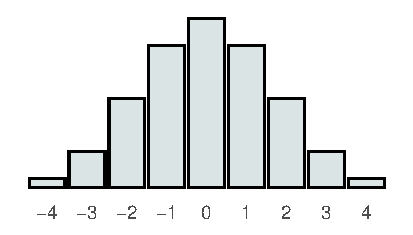
\includegraphics{stats/4dF.pdf}
\end{center}

You are unlikely to roll the extremes; you should expect to hit $\pm$4 about 1\% of the time (each)---about one time out of a hundred rolls, you should get +4, and about one time in a hundred, you should get -4. You expect to get an outcome above +3 or below -3 about 6\% of the time (each)---about one in twenty for each.

Another way to visualise the outcome of a 4dF is as the chance you have of rolling higher than some threshold value:

\begin{center}
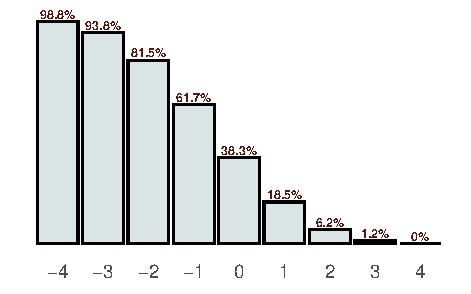
\includegraphics{stats/4dF-success.pdf}
\end{center}

To roll higher than \textbf{-4}, you just have to avoid \FudgeRes{----}, and this outcome only happens one out of 81 rolls. To roll higher than \textbf{+3} you \emph{have} to roll \FudgeRes{++++}, which also happens with probability 1/81. To roll \emph{higher} than \textbf{+4} is impossible, since this it the highest value you can roll.

In conflict resolution, this graph is relevant as it tells us how likely it is for a character without the necessary skills and relevant traits to succeed at any given difficulty rating. It is this graph of success probabilities you should have in mind when setting difficulty levels, and we return to it later. The graph, as it is here, is the probabilities you get if you had to rely on 4dF alone, without any skills or traits.


\section{Skills}
\index{Skills}

\begin{DndSidebar}[float=!t]{Skills in \emph{The Grand Casebook}}
	\subsection*{Investigation \& Knowledge}  
	\begin{itemize}
    	\item \emph{Investigate} – Analysing crime scenes, following leads, searching for hidden clues.
	    \item \emph{Lore} – Understanding history, science, the occult, and the unnatural.
	    \item \emph{Notice} – Spotting details, sensing danger, and staying aware of surroundings.
	\end{itemize}

	\subsection*{Social \& Influence}  
	\begin{itemize}
    	\item \emph{Rapport} – Gaining trust, persuading, and negotiating.
	    \item \emph{Deceive} – Lying, creating convincing cover stories, and disguises.
    	\item \emph{Provoke} – Intimidation, interrogation, and getting a reaction from others.
	    \item \emph{Contacts} – Knowing the right people, gathering information through connections.
	\end{itemize}

	\subsection*{Physical \& Dexterity}  
	\begin{itemize}
    	\item \emph{Athletics} – Running, jumping, climbing, and escaping dangerous situations.
	    \item \emph{Stealth} – Moving unseen, tailing a suspect, sneaking into restricted areas.
	    \item \emph{Fight} – Engaging in hand-to-hand combat, fencing, or using melee weapons.
	    \item \emph{Shoot} – Firearms, throwing weapons, and ranged combat.
	\end{itemize}

	\subsection*{Resilience \& Mental Fortitude}  
	\begin{itemize}
    	\item \emph{Will} – Resisting fear, staying composed under pressure, enduring mental strain.
	    \item \emph{Physique} – Strength, endurance, and the ability to withstand injury or exhaustion.
	\end{itemize}

	\subsection*{Mechanical \& Practical Skills}  
	\begin{itemize}
    	\item \emph{Burglary} – Lockpicking, safecracking, and breaking into places unseen.
	    \item \emph{Resources} – Access to wealth, favours, or valuable possessions.
	    \item \emph{Crafts} – Repairing devices, modifying tools, or working with mechanical systems.
	\end{itemize}
\end{DndSidebar}

In The Wyrd Engine, skills represent a character’s proficiency in various actions, from keen observation and quick reflexes to mastery in combat or persuasion. Whenever a character attempts a significant action where success is uncertain, they roll \textbf{4dF} and add their relevant skill modifier. The total is then compared against a \textbf{difficulty rating (DR)} set by the Game Master (GM) or an opposed roll from another character.

For player characters and most non-player characters they encounter, skills are range from \Untrained to \Expert:

\begin{DndTable}[header=Skill Levels in \emph{The Wyrd Engine}]{lX}
    \textbf{Skill Level} & \textbf{Description}\\
    \hline
    \Untrained & A character with no special training, relying on instinct or common sense. \\
    \Novice & Someone with basic knowledge or minimal hands-on experience in a skill. \\
    \Skilled & A well-trained individual who regularly practices and applies their ability. \\
    \Expert & A master in the field, capable of performing under extreme conditions. \\
\end{DndTable}

For extreme monsters, e.g., demons, dragons, or killer robots, skills might go higher. You will usually not go lower than \Untrained unless a character is impaired, e.g., drugged or recovering after severe physical or mental trauma, in which case you can.


Characters begin with a defined set of skill ranks, representing their strengths and weaknesses. Unlike systems with extensive skill lists, The Wyrd Engine keeps skills broad and flexible, allowing them to cover a wide range of related actions. For instance, a character with a high \textbf{Athletics} skill might use it to outrun pursuers, climb treacherous cliffs, or leap between rooftops. Similarly, depending on the character's background, Lore could represent expertise in ancient history, arcane knowledge, or scientific principles.

The list of skills a character can have will depend on the setting in which the game is taking place, and there is not a fixed list of skills for all Wyrd games. Generally, you should feel free to make up your own skills---remembering to keep them broad in scope---and decide between player and GM when a skill is applicable. If you like, though, you can make more detailed skill lists if that is more to your taste. In the sidebar, you can see an example of this from \emph{The Grand Casebook} setting, a Victorian/Steampunk/Gothic Horror setting.


When a character lacks a skill, they roll with a default modifier of 0, relying solely on luck and circumstance. This ensures that even untrained characters have a chance—however slim—of succeeding in tasks outside their expertise.

Let us throw the character \emph{Inspector Julian Hargrave} (see sidebar) into some difficult situations and see how he can use his skills to resolve them.

\begin{DndSidebar}[float=!t]{Example Character}
\subsection{Inspector Julian Hargrave}
\emph{Determined and methodical, Inspector Julian Hargrave is a seasoned detective. His years of experience have made him an expert at uncovering the truth, though his rigid approach sometimes clashes with the unpredictable nature of crime-solving.}
\subsubsection*{Skills}
\begin{itemize}
    \item \Expert: Investigate
    \item \Skilled: Notice, Rapport
    \item \Novice: Will, Provoke, Athletics
    \item \Untrained: Stealth, Burglary, Shoot, Resources
\end{itemize}
\end{DndSidebar}

\subsection{Skills in Action}

\subsubsection{Analysing a Crime Scene}
\begin{DndReadAloud}{}
	\textbf{Situation:} A renowned socialite has been found dead in her study. The room appears to suggest suicide, but something about the scene seems off. Julian examines the area for inconsistencies.

	\noindent
	\textbf{Difficulty Rating:} The GM decides that the difficulty rating is \Formidable – The crime scene is staged well, but subtle clues remain for an expert to notice.

	\noindent
	\textbf{Resolution:} Julian rolls \FudgeRes{++-0} and adds \textbf{+3 (Investigate)} for a total of +4. Since he exceeds the DR, he notices an overturned chair that contradicts the suicide setup. A closer look reveals a footprint near the window, suggesting an intruder.
\end{DndReadAloud}

\subsubsection{Spotting an Ambush}
\begin{DndReadAloud}{}
	\textbf{Situation:} Julian follows a suspect through the fog-laden streets when he hears an unusual shuffle behind him. Is someone trailing him?

	\noindent\textbf{Difficulty Rating:} The GM determinece that the difficulty level is \Difficult – The follower is cautious but not an expert in stealth.

	\noindent\textbf{Resolution:} Julian rolls \FudgeRes{+--0} and adds  \textbf{+2 (Notice)}, for a total of +1, meeting the DR. He catches the reflection of a blade in a shop window just in time to evade an ambush.
\end{DndReadAloud}

\subsubsection{Gaining a Witness’ Trust}
\begin{DndReadAloud}{}
	\textbf{Situation:} A frightened maid refuses to discuss her employer’s illicit dealings. Julian must convince her to cooperate.

	\noindent\textbf{Difficulty Rating:} The GM decides that the difficulty is \Challenging – She is hesitant but not impossible to persuade.

	\noindent\textbf{Resolution:} Julian rolls \FudgeRes{+---} and adds \textbf{+2 (Rapport)} for a total of +0. A tie is a failure, or is it?. If he  changes his tactics or offer protection to try again, it might turn into a partial success.
\end{DndReadAloud}

\subsubsection{Intimidating a Thief}
\begin{DndReadAloud}{}
	\textbf{Situation:} A pickpocket is caught red-handed. Instead of arresting him, Julian wants to frighten him into revealing who he works for.

	\noindent\textbf{Difficulty Rating:} The GM judges that the difficulty is \Basic – The thief is young and inexperienced but used to trouble.

	\noindent\textbf{Resolution:} Julian rolls \FudgeRes{++00} and adds \textbf{+1 (Provoke)} for a total of +3. He exceeds the DR, causing the thief to stammer out the name of a notorious smuggler before running off.
\end{DndReadAloud}

\section{Traits}
\index{Traits}

In \emph{The Wyrd Engine}, Traits represent unique abilities, specialised knowledge, or personal characteristics that distinguish characters and items from one another. Unlike skills, which define general competence, Traits provide a \emph{mechanical advantage} or \emph{narrative permission} in certain situations.

Each player character has exactly \textbf{three Traits}, carefully chosen to enhance their strengths or reflect their backstory. Non-player characters and monsters can have fewer or far more traits. Traits are broader than skills and allow a character to \emph{break} or \emph{bend} normal rules in ways that make them feel distinct.

Items can also have traits (but not skills). This is a way to add game-mechanic flavour to non-creatures and replaces weapon bonuses and similar mechanisms in other role-playing rule sets.

\subsection{How Traits Work}

Traits function in the following ways:

\begin{itemize}
    \item \textbf{Situational Bonus:} A Trait can provide a \emph{+2 bonus} to any relevant skill check if it clearly applies.
    \item \textbf{Expanded Capabilities:} A Trait may allow a character to attempt actions that others simply \emph{cannot}, such as deciphering an ancient language or crafting elaborate mechanical devices.
    \item \textbf{Once per Scene/Session Special Ability:} Some Traits grant a powerful ability that can be used once per scene or once per session, such as instantly escaping a locked room or declaring an old friend in the right place at the right time.
\end{itemize}

Traits \emph{do not stack}—if multiple Traits apply to a roll, the player must choose which one to use.

\subsection{Creating Effective Traits}

When designing Traits, they should:
\begin{itemize}
    \item Be \emph{broad} enough to be useful in multiple situations.
    \item Be \emph{specific} enough to define a unique aspect of the character.
    \item Provide a \emph{clear mechanical or narrative benefit}.
\end{itemize}

Traits can reflect personality, training, supernatural gifts, or anything else that defines a character’s abilities. Below are examples of well-crafted Traits:

\begin{DndSidebar}[float=!t]{Example Traits}
    \begin{itemize}
        \item \textbf{Master Duelist} – Gain \emph{+2 to Fight} when using a rapier or fencing techniques.
        \item \textbf{Shadow Walker} – Can move silently even in well-lit areas, allowing \emph{Stealth rolls in places others couldn’t}.
        \item \textbf{Unshakable Will} – Once per session, completely ignore the effects of fear, mind control, or intimidation.
        \item \textbf{Underworld Connections} – Gain \emph{+2 to Contacts} when dealing with criminals, smugglers, or fences.
        \item \textbf{Inventive Genius} – Can craft \emph{unique gadgets} with Crafts that would be impossible for an ordinary engineer.
    \end{itemize}
\end{DndSidebar}

\subsection{Using Traits in Play}
\begin{DndSidebar}[float=!t]{Example Character}
\subsection{Felix Cavendish}
\emph{A brilliant but erratic inventor-for-hire, Felix Cavendish is both a mechanical genius and a walking disaster. His creations are revolutionary—when they don’t explode. A rogue innovator who skirts the edges of legality, he thrives on the challenge of solving impossible problems with machines that push the limits of science.}

\subsubsection*{Skills}
\begin{itemize}
    \item \textbf{Great (+3):} Crafts
    \item \textbf{Good (+2):} Investigate, Resources
    \item \textbf{Fair (+1):} Lore, Will, Contacts
    \item \textbf{Average (+0):} Notice, Stealth, Deceive, Athletics
\end{itemize}

\subsubsection*{Traits}
\begin{itemize}
    \item \textbf{Master Tinkerer} – \emph{Gain +2 to Crafts when repairing or modifying machinery.}
    \item \textbf{Unstable Prototype} – \emph{Once per session, declare an experimental gadget with an unpredictable effect.}
    \item \textbf{A Calculated Risk} – \emph{Use Will instead of Athletics when escaping dangerous situations.}
\end{itemize}
\end{DndSidebar}
\begin{DndSidebar}[float=!b]{Example Character}
\subsection{Isadora "Isa" Lovelace}
\emph{A renowned spiritualist and occult investigator, Isa Lovelace walks the thin line between science and the supernatural. Some believe she is merely an expert in human nature, while others whisper that she truly communes with forces beyond the veil. With piercing intuition and an enigmatic presence, she seeks knowledge that others fear to uncover.}

\subsubsection*{Skills}
\begin{itemize}
    \item \textbf{Great (+3):} Empathy
    \item \textbf{Good (+2):} Investigate, Lore
    \item \textbf{Fair (+1):} Rapport, Will, Notice
    \item \textbf{Average (+0):} Stealth, Deceive, Resources, Contacts
\end{itemize}

\subsubsection*{Traits}
\begin{itemize}
    \item \textbf{A Glimpse Beyond the Veil} – \emph{Gain +2 to Empathy when sensing the emotions of the deceased.}
    \item \textbf{Foreboding Intuition} – \emph{Once per session, declare a warning based on an unseen force.}
    \item \textbf{The Cards Never Lie} – \emph{Use Lore instead of Investigate when predicting an outcome.}
\end{itemize}
\end{DndSidebar}
\begin{DndSidebar}[float=!b]{Example Character}
\subsection{Cornelius "Corny" Flint}
\emph{A silver-tongued thief and a master of misdirection, Cornelius Flint moves between high society and the criminal underworld with effortless charm. He lives by one rule—if someone is foolish enough to leave their wealth unguarded, it deserves a new owner. While he prefers to talk his way out of danger, he always has an escape plan ready when words fail.}

\subsubsection*{Skills}
\begin{itemize}
    \item \textbf{Great (+3):} Deceive
    \item \textbf{Good (+2):} Burglary, Rapport
    \item \textbf{Fair (+1):} Athletics, Stealth, Notice
    \item \textbf{Average (+0):} Contacts, Fight, Will, Resources
\end{itemize}

\subsubsection*{Traits}
\begin{itemize}
    \item \textbf{Master of Misdirection} – \emph{Gain +2 to Deceive when distracting someone in conversation.}
    \item \textbf{Sleight of Hand} – \emph{Once per session, declare you have already lifted a small item unnoticed.}
    \item \textbf{Always an Escape Plan} – \emph{Use Burglary instead of Athletics when escaping confinement.}
\end{itemize}
\end{DndSidebar}

\subsubsection{Example 1: Applying a +2 Bonus}
\begin{DndReadAloud}{}
\textbf{Situation:} Felix Cavendish, an eccentric inventor, is attempting to repair a damaged mechanical safe under a tight time limit. His player wants to use his Trait \emph{“Inventive Genius”}.

\textbf{Difficulty Rating:} The GM sets the repair difficulty at \textbf{Great (+3)}, as the damage is severe.

    \textbf{Resolution:} Felix rolls \textbf{4dF + his Crafts skill (+3)}. He rolls a result of \textbf{+1}. Normally, his total would be \textbf{+4} (Success with a Minor Cost). However, because his Trait \emph{Inventive Genius} applies, he adds an additional \textbf{+2}, bringing his final result to \textbf{+6} (Success with Style). The safe is repaired flawlessly and even runs more efficiently than before.
\end{DndReadAloud}

\subsubsection{Example 2: Expanded Capabilities}
\begin{DndReadAloud}{}
\textbf{Situation:} Isadora Lovelace, a gifted spiritualist, wants to communicate with a recently deceased victim in order to uncover clues about a murder. Normally, the \textbf{Lore} skill wouldn’t allow this.

\textbf{Trait:} \emph{“A Glimpse Beyond the Veil”} allows her to attempt supernatural interactions.

Since her Trait permits it, the GM allows a roll using \textbf{Lore}. The outcome determines how much information she can extract.
\end{DndReadAloud}

\subsubsection{Example 3: Once Per Session Ability}
\begin{DndReadAloud}{}
\textbf{Situation:} Cornelius Flint, a silver-tongued rogue, has been cornered in an alley by the city watch. Escape seems impossible.

\textbf{Trait:} \emph{“Always an Escape Plan”} allows him, once per session, to declare he had an escape route planned all along.

    \textbf{Resolution:} Instead of rolling, the GM allows him to describe a secret hatch in the alley leading to the sewers, letting him escape cleanly.
\end{DndReadAloud}
 
\subsection{Final Notes on Traits}

Traits are not just mechanical advantages; they define a character’s core competencies and role in the narrative. Players should use them creatively, and GMs should reward clever applications that fit the story.

\begin{DndComment}{Game Master Tip}
 If a player wants to use a Trait in a way that isn’t obvious, ask them to describe \emph{how} it applies. Encourage creativity while keeping balance in mind.
\end{DndComment}

\section{Gear}
\index{Gear}

Unlike other systems that track individual items, inventory weight, and resource management, \emph{The Wyrd Engine} keeps gear streamlined and abstract. Instead of worrying about encumbrance, ammunition, or minor supplies, characters only track \textbf{gear that truly matters}. This means that most mundane equipment is assumed to be available when reasonable, and only items that provide a mechanical or narrative advantage are recorded.

\subsection{Gear as Traits}
Gear in \emph{The Wyrd Engine} functions similarly to Traits. Instead of listing specific damage values or weight, an item has a \textbf{trait} that defines its benefit in play. 

Each character begins with \textbf{three pieces of gear}, and each piece should:
\begin{itemize}
    \item Provide a \emph{specific mechanical advantage} (e.g. \textbf{+2 bonus} to a relevant skill check). This works exactly the way that traits work; gear simply has traits.
    \item Offer a \emph{unique function} that enables new actions.
    \item Be \emph{narratively significant}—not just generic supplies.
\end{itemize}

See the ``Gear in \emph{The Grand Casebook}'' for examples of gear.

\begin{DndSidebar}[float=!t]{Gear in \emph{The Grand Casebook}}
\textbf{Detective’s Magnifying Glass}  
\emph{Gain +2 to Investigate when examining tiny details or analysing documents.}

\textbf{Clockwork Grappling Hook}  
\emph{Once per session, escape or reach a high place instantly.}

\textbf{Masterwork Dueling Pistol}  
\emph{Gain +2 to Shoot in one-on-one confrontations.}

\textbf{Encrypted Notebook}  
\emph{Allows the player to store complex cyphers or hidden information that only they can decode.}

\textbf{Hidden Blade}  
\emph{Use \textbf{Stealth} instead of \textbf{Fight} in a surprise attack.}

\textbf{Reinforced Trench Coat}  
\emph{Gain +2 to \textbf{Physique} when resisting blunt force trauma.}
\end{DndSidebar}

\subsection{Using Gear in Play}
Gear should not be micromanaged but used to define a character’s tools, specialities, and advantages. If an item logically fits a character’s concept—such as a detective having a notebook or a thief carrying lockpicks—it’s assumed to be available without taking up a slot. Only equipment that \emph{enhances gameplay} or \emph{creates narrative opportunities} should be explicitly listed.

\begin{DndComment}{Game Master Tip}
If a player asks, “Do I have this item?” consider whether it fits their role and background. If it makes sense, they do. If it would provide a major advantage, it should be a tracked piece of gear with a trait.
\end{DndComment}


\section{Difficulty Levels}
\index{Difficulty levels}

While \emph{The Wyrd Engine} uses a simple resolution mechanic, it is important to establish how difficult a given action is. The Game Master determines the \textbf{Difficulty Rating (DR)} based on the complexity of the task, the environment, and any obstacles the characters may face.

\subsection{Passive Opposition}
\index{Passive opposition}
The \textbf{Difficulty Rating (DR)} represents the challenge level of a task. The simplest tasks involve no active opposition—where success or failure is determined solely by the character’s own abilities. This could be deciphering an ancient cipher, scaling a rocky cliff, or crafting a delicate mechanism—situations where the only obstacle is the task itself, rather than an opposing force.

In these cases, the player rolls \textbf{4dF} + their \textbf{Skill Modifier} and applies any relevant \textbf{Trait} or \textbf{Gear bonus} (Gear Traits). If the total meets or exceeds the DR, the action succeeds.

The GM determines the difficulty rating based on two factors: how inherently challenging the task is and how critical it is to the game’s progression. A well-balanced difficulty keeps the players engaged—offering real challenges without creating dead ends. While setbacks can enrich the story, a GM should never impose an insurmountable barrier that halts progress entirely. Instead, every challenge should be an opportunity for clever thinking, teamwork, and dramatic tension.

The following table can guide you in determining the difficulty rating for a task:

\begin{DndTable}[header=Difficulty Levels in \emph{The Wyrd Engine}]{lX}
    \textbf{Difficulty Rating} & \textbf{Example Task}\\
    \hline
    \Trivial & A task so easy that failure is nearly impossible (walking across a stable floor, recalling your own name). \\
    \Simple & A straightforward action requiring minimal effort (identifying a common herb, climbing a ladder). \\
    \Easy & A minor challenge that most people can accomplish without effort (jumping over a puddle, recalling common knowledge). \\
    \Basic & An ordinary action requiring some attention (spotting a misplaced item, balancing on a narrow beam). \\
    \Challenging & A moderate test of skill or effort (spotting a hidden compartment, climbing a wooden fence). \\
    \Difficult & A task requiring training or experience (tracking footprints in the rain, persuading a sceptical guard). \\
    \Formidable & A demanding task that pushes a character’s limits (picking a complex lock under pressure, leaping between rooftops). \\
    \Arduous & A near-impossible feat requiring mastery (detecting a forged document at a glance, sniping a target from extreme range). \\
    \Extreme & A task on the edge of human capability (convincing a lifelong enemy to trust you, performing surgery in total darkness). \\
    \Impossible & A superhuman achievement defying all odds (dodging bullets mid-air, convincing an ancient dragon to surrender). \\
\end{DndTable}

For levels up to \Basic, rolls are usually unnecessary unless dramatic tension is involved. For characters with appropriate skills, \Basic tasks can also be handled without rolls.

We can superimpose the difficulty levels on the 4dF success rate graph to directly visualise how difficult it will be with just dice rolls to reach a given level:

\begin{center}
	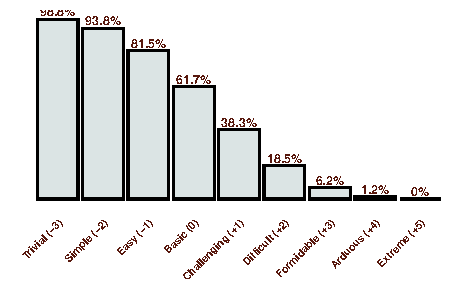
\includegraphics{stats/4dF-DR.pdf}
\end{center}

The graph tells us that even \Trivial tasks can fail if you are unskilled and unlucky enough, and \Challenging tasks will fail a third of the time for someone without the necessary skills.

Adding skills effectively shifts the difficulty levels. When playing the game, we add skill levels to the 4dF rolls, as this is the easiest way to calculate the result, but when setting difficulty levels, it is easier to think in terms of how difficult an unskilled character would find a task, and then shift the difficulty levels down by one for each skill level a character has.

A skill level of \Novice adds one to the 4dF, which effectively shifts the difficulties down by one. If we are adding \textbf{+1} to a roll, the unmodified range of \textbf{-4} to \textbf{+4} for a \Untrained character instead becomes the shifted range of \textbf{-3} to \textbf{+5}, for example. With this switch, the difficulty with which a \Novice character hits a \Challenging level will be the same as if he only had to reach the \Basic level.

\begin{center}
	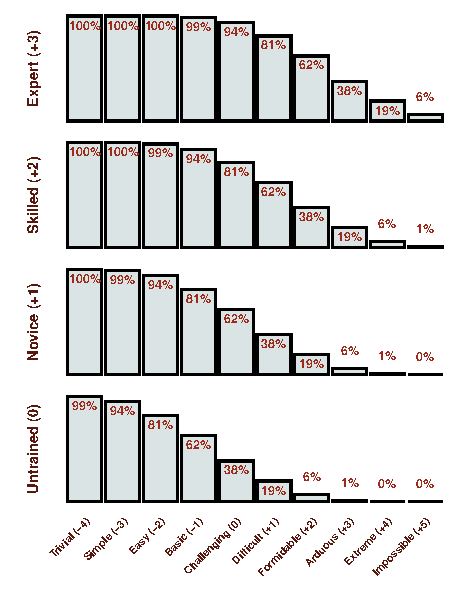
\includegraphics{stats/shifted-DR.pdf}
\end{center}

A \Basic task, which has a 2/3 chance of success for an \Untrained character will be a success one out of twenty for a \Novice and a guaranteed success for an \Expert character. An \Extreme task, which will be impossible for an \Untrained and not much easier for a \Novice, has a one-in-five chance of success for an \Expert. Add in a \textbf{Trait (+2)}---which shifts the range by an additional two points---and an \Expert character will, under the right circumstances, have a one-in-three chance of doing the impossible.

The table below shows the probability of success for the different difficulty levels at different skill levels:

\begin{DndTable}[header=Success probability per skill level]{lrrrr}
    \textbf{Difficulty} & \textbf{0} & \textbf{+1} & \textbf{+2} & \textbf{+3} \\
    \hline
    \Trivial     & 98.8\% & 100.0\% & 100.0\% & 100.0\% \\
    \Simple      & 93.8\% &  98.8\% & 100.0\% & 100.0\% \\
    \Easy        & 81.5\% &  93.8\% &  98.8\% & 100.0\% \\
    \Basic       & 61.7\% &  81.5\% &  93.8\% & 98.8\% \\
    \Challenging & 38.7\% &  61.7\% &  81.5\% & 93.8\% \\
    \Difficult   & 18.5\% &  38.7\% &  61.7\% & 81.5\% \\
    \Formidable  &  6.2\% &  18.5\% &  38.7\% & 61.7\% \\
    \Arduous     &  1.2\% &   6.2\% &  18.5\% & 38.7\% \\
    \Extreme     &  -     &   1.2\% &   6.2\% & 18.5\% \\
    \Impossible  &  -     &   -     &   1.2\% &  6.2\% \\
\end{DndTable}

Players will not need to consult this table during a game---in \emph{The Wyrd Engine} we are not keen on using tables for game mechanics---but it should give a Game Master a rough idea of how to set difficulty levels when planning a game session.


\begin{DndComment}{Game Master Tip}
	When deciding on difficulty levels, you should focus on the narrative aspects of the game rather than realism in difficulty. You want to give the players exciting challenges, but any conflict resolution should have narrative relevance. Don't ask for dice rolls if you can act out a scene instead, and don't ask for dice rolls unless both failure and success will have exciting consequences. It is okay to have automatic wins and automatic losses if the alternative will break the story you are trying to tell, and it is okay to set unrealistically low or high difficulty levels if that is what it takes to tell a good story.
	\end{DndComment}



\subsection{Active Opposition}
\index{Active opposition}
When two characters compete directly but are not in combat (for that, see below), both roll \textbf{4dF + their relevant skill}. The highest result wins.

\begin{itemize}
    \item If one character beats the other by \textbf{1 or 2 points}, they succeed with a minor advantage.
    \item If they beat the other by \textbf{3 or more points}, their success is so impressive that the GM can, at their discretion, provide the winning character with a \textbf{boon}.
\end{itemize}

A \textbf{boon} is a one-use trait invented for the situation at hand. It is only active for the current scene and is lost if not used after the scene ends.

\subsection{Ties and Partial Successes}
\index{Ties}\index{Partial successes}
Not every roll results in a clean success or failure. When a roll \textbf{ties} the Difficulty Rating, or when failure would halt progress entirely, the GM may introduce a \textbf{complication}:

\begin{itemize}
    \item \textbf{Success with a Cost:} The action succeeds, but at a price (e.g., escaping a pursuer but losing an important clue).
    \item \textbf{Mixed Success:} The character achieves part of their goal, but not completely (e.g., unlocking a door but setting off an alarm).
    \item \textbf{A New Complication:} The failure introduces an unexpected twist (e.g., picking a lock only to find guards already inside).
\end{itemize}

\subsection{Interpreting Failure}
\index{Interpreting failure}
A failed roll doesn’t necessarily mean the character is incompetent—it simply means their approach didn’t work this time. The GM should ensure failures lead to new choices, not dead ends.

\begin{DndComment}{Game Master Tip}
    If a failed roll would stop the story in its tracks, offer the player an alternative: “You can still succeed but at a cost.” This keeps the momentum going while making failure meaningful.
\end{DndComment}

\subsection{Boosts: Optional Rule for Increasing Success}\index{Boosts}

As an optional rule, you can allow players to create \textbf{Boosts}—temporary numerical bonuses such as +1 or +2 that can be applied to a relevant roll. Boosts represent situational advantages, quick thinking, or clever tactics that enhance a character’s chance of success.  

Boosts can take different forms, including:  

\begin{itemize}
    \item \textbf{Preparation}: Taking extra time to study a problem, setting up tools, or laying a trap.  
    \item \textbf{Tactical Advantage}: Gaining higher ground, flanking an enemy, or exploiting a distraction.  
    \item \textbf{Environmental Factors}: Using dim lighting for stealth, a rainstorm to obscure movement, or an echoing chamber to amplify a command.  
    \item \textbf{Teamwork}: Coordinating efforts with allies, assisting with a skill check, or providing cover in combat.  
\end{itemize}

To gain a Boost, a player must describe how their actions create an advantage and roll an appropriate skill or trait check. If successful, they gain a Boost that applies to their next relevant roll. Boosts typically last for a single action but may persist longer if narratively justified.  

Boosts are a simple way to reward creativity, reinforce teamwork, and give players more control over their success in \textit{The Wyrd Engine}.


\subsection{Teamwork: Optional Rule for Assisting Allies}

In \textit{The Wyrd Engine}, collaboration can be just as important as individual skill. As an optional rule, players may assist one another to increase the chances of success in a task or conflict. When a character helps an ally, they provide a \textbf{Teamwork Bonus}, a small numerical boost that enhances the primary actor’s roll.  

Teamwork Bonuses can take different forms, including:  

\begin{itemize}
    \item \textbf{Direct Assistance}: Actively working alongside an ally, such as two people lifting a heavy object or multiple minds solving a puzzle.  
    \item \textbf{Tactical Coordination}: Calling out enemy movements in battle, providing covering fire, or distracting an opponent.  
    \item \textbf{Shared Knowledge}: Using past experiences or expertise to guide another character’s actions, such as an engineer giving instructions to a less skilled mechanic.  
    \item \textbf{Moral Support}: Bolstering an ally’s resolve with encouragement, inspiration, or leadership.  
\end{itemize}

To assist, the supporting player must describe how they are helping and roll an appropriate skill or trait check. If successful, they grant the primary actor a \textbf{+1 bonus} to their roll. In special cases—such as exceptional teamwork, well-planned strategies, or group efforts—the GM may allow the bonus to increase to \textbf{+2}.  

Only one character can provide a Teamwork Bonus per roll unless the GM rules that multiple participants are required. This system encourages cooperation and allows players to combine their strengths to overcome greater challenges.

\section{Basic Combat in The Wyrd Engine}
\index{Combat}

Combat in \textit{The Wyrd Engine} is designed to be fast, cinematic, and deadly. Instead of tracking minute details like hit points or exact damage values, the system focuses on the flow of action, player choices, and the consequences of combat.

\subsection{Initiative: Who Acts First?}
\index{Combat!Initiative} 

Combat follows a structured yet flexible turn order:

\begin{DndReadAloud}{Determining Initiative}
\begin{itemize}
    \item \textbf{Surprise \& Readiness:} If one side is clearly ambushing the other, they act first.
    \item \textbf{Tactical Positioning:} If no clear ambush is present, the GM determines turn order based on readiness.
    \item \textbf{Rolling for Initiative:} If multiple characters are competing to act first, roll \textbf{4dF + Notice} (or another relevant skill). The highest roll acts first, with ties resolved narratively.
\end{itemize}
\end{DndReadAloud}

\subsection{Taking Actions in Combat}
\index{Combat actions}

On their turn, a character can do the following:
\begin{itemize}
    \item \textbf{One primary action} (Attack, defend, use an item, complex manoeuvre)
    \item \textbf{One minor action} (Draw a weapon, reposition, open a door, shout a command)
    \item \textbf{Free actions} (Speaking briefly, minor environmental interactions)
\end{itemize}

\subsection{Attacking and Defending}
\index{Combat!Attacking}\index{Combat!Defending}

Attacks are resolved using opposed rolls:
\begin{DndReadAloud}{Attack Resolution}
\begin{itemize}
    \item The attacker rolls \textbf{4dF + their combat skill} (\textbf{Fight} for melee, \textbf{Shoot} for firearms).
    \item The defender rolls \textbf{4dF + their defense skill} (\textbf{Athletics} for dodging, \textbf{Fight} for parrying).
    \item If the attacker’s total exceeds the defender’s, the attack lands and deals damage.
\end{itemize}
\end{DndReadAloud}

\index{Damage}
\index{Combat!Soaking up damage}
The damage inflicted must be soaked up by either \textbf{Stress} or \textbf{Wounds}. Depending on the setting, you can scale the damage to stress/wound conversion. Converting damage to stress or wounds 1-to-1 gives you a realistic but rather deadly game, so for more action-packed swashbuckling adventures, you might want to convert them 2-to-1 or 3-to-1.

\begin{DndSidebar}[float=!t]{Example Attack}
Jonathan Blackwood swings a cane at an enemy thug. He rolls \textbf{4dF +2 (Fight)}, while the thug rolls \textbf{4dF +1 (Athletics)} to dodge. If Jonathan’s result is higher, the hit lands.
\end{DndSidebar}


\subsection{Damage: Stress and Wounds}
\index{Damage}

Instead of traditional hit points, \textit{The Wyrd Engine} uses \textbf{Stress}\index{Damage!Stress}\index{Stress} for minor injuries and \textbf{Wounds}\index{Damage!Wounds}\index{Wounds} for lasting harm.

\begin{DndReadAloud}{Stress and Wounds}
\begin{itemize}
    \item \textbf{Stress:} Represents minor setbacks, fatigue, or temporary injuries. Every character has \textbf{five Stress boxes}. These are automatically cleared after a fight.
    \item Once all stress boxes are filled, additional damage results in \textbf{Wounds}.
\end{itemize}
\end{DndReadAloud}

Damage is converted to wounds similarly to how damage is converted to stress, using 1-to-1 or some other conversion factor. A \textbf{Mild Wound} absorbs the same as one stress box, a \textbf{Moderate Wound} the same as two stress boxes, and a \textbf{Severe Wound} the same as three stress boxes. In addition, when taking a \textbf{Wound}, one or more relevant skills are affected.

\begin{DndTable}[header=]{ll}
    \textbf{Wound Type} & \textbf{Effect} \\
    \hline
    \textbf{Mild Wound}  & -1 to relevant skill rolls \\
    \textbf{Moderate Wound} & -2 to relevant skill rolls \\
    \textbf{Severe Wound}  & -3 to all physical actions \\
\end{DndTable}

Damage does not have to fill a wound to invoke it. If a character already has a \textbf{Mild Wound} and takes \textbf{+1} in damage, it goes into the \textbf{Moderate Wound} \emph{and fills it}. Even though a \textbf{Moderate Wound} can take two in damage, it is inflicted as soon as it takes \emph{any} damage, and if the \textbf{+1} cannot go into a stress box or the \textbf{Mild Wound}, it goes into the \textbf{Moderate Wound}.

\begin{DndSidebar}[float=!t]{Example Wound}
Josephine Langley is shot during a gunfight and takes \textbf{+2} damage. She has no remaining Stress boxes, so she takes a \textbf{Moderate Wound} (since a \textbf{Moderate Wound} can soak up two damage while a \textbf{Mild Wound} cannot). The GM rules that the injury impairs her movement, applying a \textbf{-2} penalty to \textbf{Athletics} and \textbf{Fight} rolls.
\end{DndSidebar}

If all stress boxes are filled and all three wounds are taken, the character is out of action. What this means is up to the GM, but games are usually more fun if player characters live to fight another day. For one-shot games, it is okay to kill off characters towards the end of the session, but don't do it early in the game.

\subsection{Healing and Recovery}
\index{Healing}\index{Recovery}

\begin{itemize}
    \item \textbf{Stress} clears at the end of a scene.
    \item \textbf{Mild Wounds} require a short rest (a few hours) or first aid.
    \item \textbf{Moderate Wounds} require days of rest or professional medical care.
    \item \textbf{Severe Wounds} require weeks of rest, surgery, or supernatural healing (if applicable).
\end{itemize}

\subsection{Combat Maneuvers and Special Actions}
Instead of simply attacking, players can use tactical manoeuvres:

\begin{DndReadAloud}{Combat Maneuvers}
\begin{itemize}
    \item \textbf{Disarm:} Use Fight to knock a weapon from an opponent’s hands.
    \item \textbf{Grapple:} Use Fight vs. Athletics to restrain an enemy.
    \item \textbf{Push:} Use Athletics to shove an opponent into hazards.
    \item \textbf{Feint:} Use Deceive to trick an enemy into missing a defense.
    \item \textbf{Suppressing Fire:} Use Shoot to force enemies into cover.
    \item \textbf{Intimidate:} Use Provoke to demoralize foes.
\end{itemize}
\end{DndReadAloud}

\emph{The Wyrd Engine} does not have rules for all the myriad ways that actions can be used in combat, but the GM should generally try to convert an action into either an unopposed or opposed obstacle and let the outcome affect bonuses and penalties for future dice rolls.

\subsection{Weapons and Gear in Combat}
Weapons do not deal numeric damage but affect combat through \textbf{Traits}. Weapon traits work the same way as any gear trait and can be used when attacking or defending.

\begin{DndReadAloud}{Types of Weapon Traits}
\begin{itemize}
    \item \textbf{Weapons with Traits} grant \textbf{+2} in relevant situations (e.g., “Mastercrafted Rapier” gives +2 to Fight in duels).
    \item \textbf{Firearms} can inflict instant Wounds if the shot is well-placed.
    \item \textbf{Improvised Weapons} may impose a penalty unless the character is skilled in their use.
\end{itemize}
\end{DndReadAloud}

When a weapon's \textbf{Trait} adds to the attack of a character, it will indirectly affect the damage the attack is inflicting. More interesting uses of weapon traits give other advantages to their wielder.

\begin{DndReadAloud}{Example Weapon Traits}
\begin{itemize}
    \item \textbf{Fine Dueling Sabre} – \textit{+2 to Fight when dueling.}
    \item \textbf{Hidden Derringer} – \textit{Once per scene, draw a concealed firearm unnoticed.}
    \item \textbf{Reinforced Cane} – \textit{Can be used as both a weapon and a defensive tool.}
\end{itemize}
\end{DndReadAloud}

\section{Death and the End of Combat}
When a character suffers a \textbf{Severe Wound} and takes further damage, they are at risk of death. The GM may allow:
\begin{itemize}
    \item A final desperate action before succumbing.
    \item A chance to survive if an ally intervenes.
    \item A dramatic consequence, such as permanent injury.
\end{itemize}

Combat ends when one side is defeated, flees, or surrenders. Survivors must then deal with the consequences of their wounds, the choices they made, and the path ahead.

\begin{DndComment}{Game Master Tip}
If a player is at risk of death, consider narrative consequences rather than instant removal. A major wound or permanent injury can be more interesting than a sudden death.
\end{DndComment}


\section{Character Creation}
\index{Character creation}

Creating a character in \textbf{The Wyrd Engine} is a quick and streamlined process, designed to get players into the game with minimal preparation. Each character is defined by a small but meaningful set of attributes that shape their role in the story. Unlike systems with long-term progression, \textbf{The Wyrd Engine} prioritises narrative impact over mechanical advancement, making character creation simple yet flexible.

Every player character is built using the following elements:

\subsection{Step 1: Concept}

Before assigning mechanics, players should develop a brief \textbf{character concept}. This is a short description of who the character is, their role in the story, and what makes them interesting. Concepts should be evocative but flexible, helping guide both roleplay and mechanical choices.

\begin{DndSidebar}[float=!t]{Example Character Concepts}
    \begin{itemize}
        \item \emph{A disgraced noble turned detective, haunted by his past.}
        \item \emph{An eccentric engineer whose inventions are as brilliant as they are dangerous.}
        \item \emph{A silver-tongued con artist who survives by wit and charm.}
        \item \emph{A fearless occult investigator seeking forbidden knowledge.}
    \end{itemize}
\end{DndSidebar}

\subsection{Step 2: Choose Skills}

Each character has a set of \textbf{Skills} that determine their strengths and weaknesses. Skills represent broad areas of expertise rather than hyper-specialised talents, ensuring versatility.

Characters receive a total of \textbf{six skill ranks}, distributed as follows:

\begin{itemize}
    \item \textbf{1 Great (+3)} skill
    \item \textbf{2 Good (+2)} skills
    \item \textbf{3 Fair (+1)} skills
\end{itemize}

All unselected skills default to \textbf{+0}.

\begin{DndReadAloud}{}
When assigning skills, players should consider their character’s background and expertise. A veteran detective might prioritise \textbf{Investigate} and \textbf{Notice}, while a rogue might favour \textbf{Stealth} and \textbf{Deceive}.
\end{DndReadAloud}

The total sum of skill ranks must always equal \textbf{10}. This ensures that every character is balanced in overall competence while allowing for specialisation.

\subsection{Step 3: Select Traits}

Every character has exactly \textbf{three Traits}. Traits represent exceptional abilities, personal quirks, or special training that set a character apart. 

\textbf{Traits provide one of three benefits:}
\begin{itemize}
    \item A \textbf{+2 bonus} when applied to a relevant skill check.
    \item A \textbf{special ability} that can be used \emph{once per scene or session}.
    \item A \textbf{narrative permission} to attempt actions that would normally be impossible.
\end{itemize}

\begin{DndSidebar}[float=!b]{Example Traits}
    \begin{itemize}
        \item \textbf{Master Duelist} – \emph{Gain +2 to Fight when using a rapier or fencing techniques.}
        \item \textbf{Inventive Genius} – \emph{Can craft unique gadgets that defy conventional mechanics.}
        \item \textbf{Unshakable Will} – \emph{Once per session, ignore the effects of fear or mind control.}
        \item \textbf{Underworld Connections} – \emph{Gain +2 to Contacts when dealing with criminals.}
        \item \textbf{The Cards Never Lie} – \emph{Use Lore instead of Investigate when predicting an outcome.}
    \end{itemize}
\end{DndSidebar}

Traits should enhance a character’s strengths and provide unique advantages in play. They should not be overly broad or cover multiple unrelated areas.

\subsection{Step 4: Select Gear}

\textbf{The Wyrd Engine} does not track mundane items or encumbrance. Instead, characters select \textbf{three pieces of notable gear} that have a mechanical or narrative impact.

Each piece of gear functions like a Trait, providing either:
\begin{itemize}
    \item A \textbf{+2 bonus} when used appropriately.
    \item A \textbf{special ability} usable once per scene or session.
    \item A \textbf{narrative permission} to perform unique actions.
\end{itemize}

\begin{DndSidebar}[float=!t]{Example Gear}
    \begin{itemize}
        \item \textbf{Clockwork Lockpick} – \emph{+2 to Burglary when opening mechanical locks.}
        \item \textbf{Enchanted Mirror} – \emph{Once per session, reveal a hidden truth.}
        \item \textbf{Mastercrafted Rapier} – \emph{+2 to Fight in one-on-one duels.}
        \item \textbf{Detective’s Notebook} – \emph{Use Investigate instead of Rapport when questioning suspects.}
        \item \textbf{Hidden Derringer} – \emph{Once per scene, draw a concealed firearm unnoticed.}
    \end{itemize}
\end{DndSidebar}

\subsection{Step 5: Define Stress and Consequences}

Characters have a limited ability to absorb harm before suffering long-term effects.

\begin{itemize}
    \item \textbf{Three Stress Boxes} – Used to absorb minor failures.
    \item \textbf{Mild, Moderate, and Severe Wounds} – Represent lasting harm or setbacks.
\end{itemize}

Wounds replace traditional hit points and can reflect physical, mental, or social strain. A "Mild" consequence might be a bruised rib, while a "Severe" consequence could be a permanent injury or a shattered reputation.

\subsection{Step 6: Final Details}

With mechanics in place, players can now define their character’s:
\begin{itemize}
    \item \textbf{Name} – Fitting for the setting and character concept.
    \item \textbf{Appearance} – Distinctive traits, clothing, and demeanour.
    \item \textbf{Personality} – Key personality traits, motivations, or quirks.
    \item \textbf{Backstory} – A brief origin story or notable past experiences.
\end{itemize}

\begin{DndComment}{Final Advice for Players}
\textbf{Focus on character over numbers.} The Wyrd Engine is designed for narrative-driven play, so build a character that fits the story rather than optimising for maximum efficiency.
\end{DndComment}

Once these steps are complete, the character is ready for play!



